\section{Temporal Validation Results}
\label{sec:5_5}

Expanding window validation assesses model stability and data requirements across time.

\begin{figure}[htbp]
    \centering
    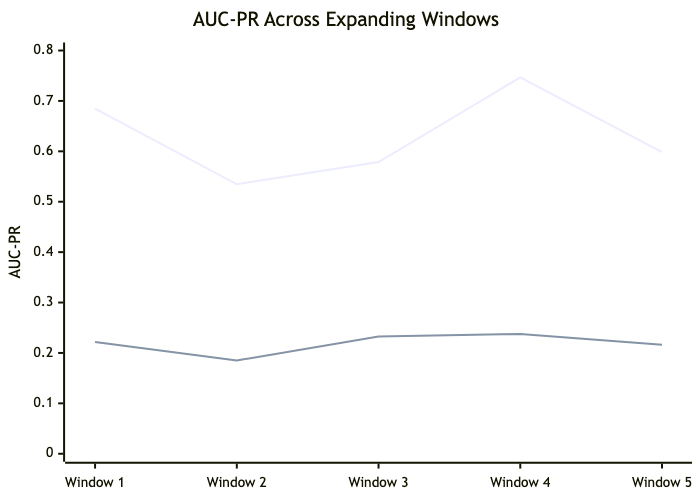
\includegraphics[width=0.8\textwidth]{figures/fig_5_5_5_1.png}
    \caption{AUC-PR Across Expanding Windows}
    \label{fig:5_5}
\end{figure}

\begin{table}[htbp]
    \centering
    \caption{Expanding Window Results}
    \label{tab:5_6}
    \begin{tabular}{lcccc}
        \toprule
        Window & Train End & Training Samples & XGB AUC-PR & GNN+XGB AUC-PR \\
        \midrule
        1 & 2025-01-30 & 103,018 & 0.6846 & 0.2219 \\
        2 & 2025-03-01 & 173,739 & 0.5346 & 0.1850 \\
        3 & 2025-03-31 & 240,660 & 0.5788 & 0.2325 \\
        4 & 2025-04-30 & 308,071 & 0.7467 & 0.2376 \\
        5 & 2025-05-30 & 373,484 & 0.5982 & 0.2164 \\
        \midrule
        \textbf{Mean} & — & — & \textbf{0.6286 $\pm$ 0.077} & 0.2187 $\pm$ 0.018 \\
        \bottomrule
    \end{tabular}
\end{table}

\textbf{Key Findings:}

\begin{itemize}
    \item \textbf{Catastrophic GNN Degradation:} GNN+XGBoost exhibits severe performance collapse in expanding window validation (mean AUC-PR 0.2187), representing a \textbf{70\% degradation} compared to fixed split performance (0.733, Table~\ref{tab:5_1}). This catastrophic failure indicates GNN embeddings are highly sensitive to temporal distribution shifts in graph structure.

    \item \textbf{Vanilla XGBoost Temporal Stability:} In contrast, tabular-only XGBoost maintains reasonable performance (mean 0.6286 $\pm$ 0.077), achieving 86\% of its fixed-split performance. This demonstrates greater robustness to evolving fraud patterns when using attribute-only features.

    \item \textbf{Graph Structure Non-Stationarity:} The GNN failure suggests that entity-sharing networks (device, IP, email, phone) evolve rapidly over time. New fraud rings form distinct graph components not represented in training data, causing learned GNN aggregation functions to extrapolate poorly. Tabular features (screen resolution, payment mode, listing price) exhibit more stable distributions.

    \item \textbf{Concept Drift:} Vanilla XGBoost shows drift range of 0.21 (max 0.7467 in Window 4, min 0.5346 in Window 2), with notable performance dip in March 2025. This temporal variation motivates frequent retraining schedules (monthly recommended).
\end{itemize}

\textbf{Production Implications:} This analysis reveals a critical limitation of graph-based fraud detection: while GNN embeddings provide supplementary signal in fixed-split evaluation (+17.3\% feature importance, Section~\ref{sec:5_9}), they demonstrate poor generalization under temporal distribution shift. For operational deployment with incremental retraining, \textbf{Vanilla XGBoost is strongly recommended} over GNN+XGBoost due to:
\begin{enumerate}
    \item Superior temporal robustness (0.63 vs 0.22 mean AUC-PR in expanding windows)
    \item Lower computational cost (no graph construction or GNN training required)
    \item Simpler deployment (no need to maintain entity-relationship graphs)
\end{enumerate}

GNN-augmented approaches may be viable only with: (1) very large, stable datasets ($>$300K samples), (2) static graph topology, or (3) graph-aware continual learning strategies to adapt to structural evolution. Future work should investigate temporal graph neural networks (e.g., ROLAND \cite{you2022roland}) designed for non-stationary graphs.
